
%(BEGIN_QUESTION)
% Copyright 2010, Tony R. Kuphaldt, released under the Creative Commons Attribution License (v 1.0)
% This means you may do almost anything with this work of mine, so long as you give me proper credit

Anta at denne magnetventilstyrte ventilen står åpen hele tiden, uansett hvilken bryter som trykkes:

$$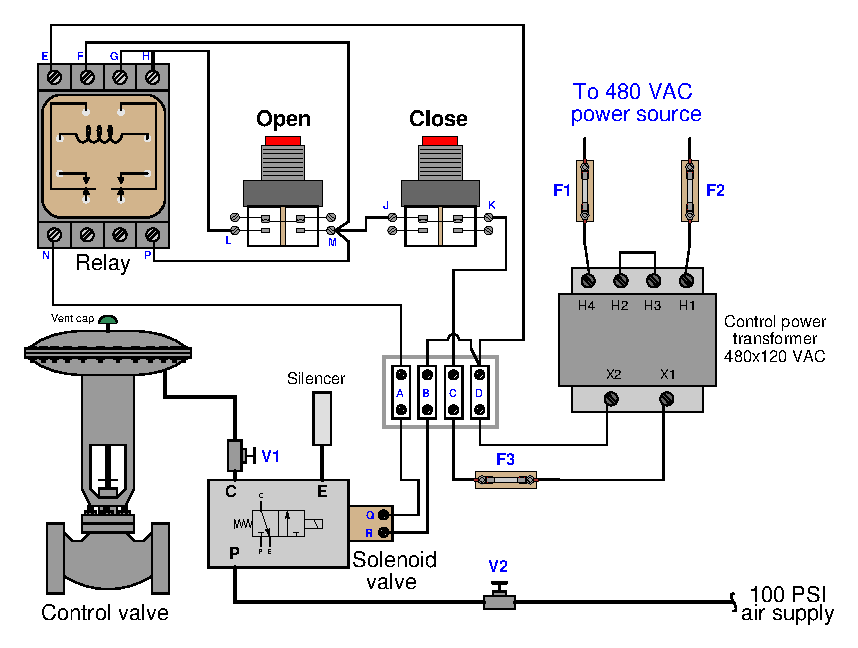
\includegraphics[width=15.5cm]{i01425x01.eps}$$

Du måler 474 volt mellom terminal {\bf H1} og {\bf H4} på transformatoren, og 118 volt mellom terminal {\bf M} og {\bf D}, med begge trykknappbryterne upåvirket.

Vurder sannsynligheten for hver av de spesifiserte feilene i dette systemet. Vurder hver feil én om gangen (det vil si ingen samtidige feil), og avgjør om hver feil alene kan forklare {\it alle} målinger og symptomer i systemet. Oppgi også én ekstra mulig feil som ikke er listet i tabellen.

% No blank lines allowed between lines of an \halign structure!
% I use comments (%) instead, so that TeX doesn't choke.

$$\vbox{\offinterlineskip
\halign{\strut
\vrule \quad\hfil # \ \hfil & 
\vrule \quad\hfil # \ \hfil & 
\vrule \quad\hfil # \ \hfil \vrule \cr
\noalign{\hrule}
%
% First row
{\bf Feil} & {\bf Mulig} & {\bf Umulig} \cr
%
\noalign{\hrule}
%
% Another row
Sikring F3 utløst (feilet åpen) &  &  \cr
%
\noalign{\hrule}
%
% Another row
Magnetspole feilet åpen &  &  \cr
%
\noalign{\hrule}
%
% Another row
``Open''-bryterkontakter (L til M) feilet åpen &  &  \cr
%
\noalign{\hrule}
%
% Another row
``Close''-bryterkontakter (J til K) feilet kortsluttet &  &  \cr
%
\noalign{\hrule}
%
% Another row
Reléspole feilet kortsluttet &  &  \cr
%
\noalign{\hrule}
%
% Another row
Relékontakt (G til P) feilet kortsluttet &  &  \cr
%
\noalign{\hrule}
%
% Another row
Relékontakt (F til N) feilet kortsluttet &  &  \cr
%
\noalign{\hrule}
%
% Another row
Ledningsbrudd mellom terminal K og D &  &  \cr
%
\noalign{\hrule}
%
% Another row
Ventil V1 stengt &  &  \cr
%
\noalign{\hrule}
%
% Another row
Ventil V2 stengt &  &  \cr
%
\noalign{\hrule}
} % End of \halign 
}$$ % End of \vbox

Til slutt: Angi den {\it neste} diagnostiske testen eller målingen du ville gjort på systemet. Forklar hvordan resultatet av denne testen eller målingen bidrar til å identifisere feilens plassering og/eller natur videre.

\underbar{file i01425}
%(END_QUESTION)





%(BEGIN_ANSWER)

% No blank lines allowed between lines of an \halign structure!
% I use comments (%) instead, so that TeX doesn't choke.

$$\vbox{\offinterlineskip
\halign{\strut
\vrule \quad\hfil # \ \hfil & 
\vrule \quad\hfil # \ \hfil & 
\vrule \quad\hfil # \ \hfil \vrule \cr
\noalign{\hrule}
%
% First row
{\bf Feil} & {\bf Mulig} & {\bf Umulig} \cr
%
\noalign{\hrule}
%
% Another row
Sikring F3 utløst (feilet åpen) &  & $\surd$ \cr
%
\noalign{\hrule}
%
% Another row
Magnetspole feilet åpen &  & $\surd$ \cr
%
\noalign{\hrule}
%
% Another row
``Open''-bryterkontakter (L til M) feilet åpen &  & $\surd$ \cr
%
\noalign{\hrule}
%
% Another row
``Close''-bryterkontakter (J til K) feilet kortsluttet & $\surd$ &  \cr
%
\noalign{\hrule}
%
% Another row
Reléspole feilet kortsluttet &  & $\surd$ \cr
%
\noalign{\hrule}
%
% Another row
Relékontakt (G til P) feilet kortsluttet &  & $\surd$ \cr
%
\noalign{\hrule}
%
% Another row
Relékontakt (F til N) feilet kortsluttet & $\surd$ &  \cr
%
\noalign{\hrule}
%
% Another row
Ledningsbrudd mellom terminal K og D &  & $\surd$ \cr
%
\noalign{\hrule}
%
% Another row
Ventil V1 stengt & ? &  \cr
%
\noalign{\hrule}
%
% Another row
Ventil V2 stengt &  & $\surd$ \cr
%
\noalign{\hrule}
} % End of \halign 
}$$ % End of \vbox

For at en ``stengt'' V1 skal kunne forklare at reguleringsventilen står åpen hele tiden, måtte den håndventilen blitt stengt mens systemet var i en helt bestemt tilstand! Å stenge V1 under {\it vilkårlige} forhold vil ikke nødvendigvis gi denne effekten.

\vskip 10pt

En god ``neste test'' er å måle spenning mellom terminal Q og R på magnetspolen.

%(END_ANSWER)





%(BEGIN_NOTES)

Ytterligere mulige feil som ikke er listet i tabellen, inkluderer:

\begin{itemize}
\item{} Kortslutning mellom terminal A og C 
\item{} Kraftig tilstoppet lyddemper
\end{itemize}









\vskip 20pt \vbox{\hrule \hbox{\strut \vrule{} {\bf Virtuell feilsøking} \vrule} \hrule}

Dette spørsmålet egner seg godt som en ``Virtuell feilsøking''-øvelse. Når du presenterer diagrammet for studentene, forestiller du deg først en bestemt feil i systemet. Deretter presenterer du ett eller flere symptomer på denne feilen (noe en operatør eller annen bruker kan observere). Studentene foreslår så ulike diagnostiske tester for å identifisere feilens natur og plassering, slik teknikere ville gjort i praktisk feilsøking. Din oppgave er å fortelle hva resultatet ville blitt for hver foreslått test, og dokumentere resultatene slik at alle studentene kan se dem.

Under og etter øvelsen er det nyttig å stille oppfølgingsspørsmål som:

\begin{itemize}
\item{} Hva forteller resultatet av den siste diagnostiske testen deg om feilen?
\item{} Anta at resultatene av den siste diagnostiske testen var annerledes. Hva ville det resultatet fortalt deg om feilen?
\item{} Er den siste diagnostiske testen den beste vi kunne gjort?
\item{} Hva ville vært ideell testrekkefølge for å diagnostisere problemet i færrest mulig trinn?
\end{itemize}


%INDEX% Troubleshooting review: electric circuits

%(END_NOTES)

